% -*- coding: utf-8 -*-

\documentclass[b5paper,papersize,tombow,12pt]{jsbook}

\usepackage{amsmath,ascmac}
\usepackage{graphicx}
\usepackage{lettrine}
\usepackage{fancyhdr}
% Palatino
\usepackage{palatino}


%% Page Layout
% B5: 182mm x 257mm
\setlength{\voffset}{0mm}
\setlength{\topmargin}{-15mm}
\setlength{\textheight}{29\Cvs}
\setlength{\footskip}{10mm}

% set margin for openleft
% \setlength{\oddsidemargin}{-\oddsidemargin}
% \setlength{\evensidemargin}{-\oddsidemargin}


\pagestyle{fancy}

\fancyhead{}
% \fancyhead[RO,RE]{\rightmark}
% \fancyhead[LE,LO]{\leftmark}
\fancyhead[RO]{\rightmark}
\fancyhead[LE]{\leftmark}
\cfoot{\bfseries -- \thepage \ --} % page number at the center bottom
\renewcommand{\headrule}{
\vskip -1.5mm
\hskip-0.03\textwidth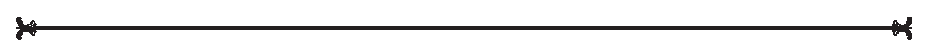
\includegraphics[width=1.06\textwidth,height=3.78mm]{hayamiz/images/hrule.eps}
\vskip -2.28mm
}

% jsbook.cls use 'plainhead' style for the first page of each chapter
\fancypagestyle{plainhead}{
\fancyhf{}
\cfoot{\bfseries -- \thepage \ --}
\renewcommand{\headrulewidth}{0.0pt}
\renewcommand{\headrule}{}
}

% jsbook.cls use 'empty' style for blank
\fancypagestyle{empty}{
\fancyhf{}
\cfoot{\bfseries -- \thepage \ --}
\renewcommand{\headrulewidth}{0.0pt}
\renewcommand{\headrule}{}
}

\makeatletter
\renewcommand{\chapter}{%
  \if@openright\cleardoublepage\else\clearpage\fi
  \plainifnotempty % 元: \thispagestyle{plain}
  \global\@topnum\z@
  \if@english \@afterindentfalse \else \@afterindenttrue \fi
  \secdef\@chapter\@schapter}
\def\@chapter[#1]#2{%
  \ifnum \c@secnumdepth >\m@ne
    \if@mainmatter
      \refstepcounter{chapter}%
      \typeout{\@chapapp\thechapter\@chappos}%
      \addcontentsline{toc}{chapter}%
        {\protect\numberline
        {\if@english\thechapter\else\@chapapp\thechapter\@chappos\fi}%
        #1}%
    \else\addcontentsline{toc}{chapter}{#1}\fi
  \else
    \addcontentsline{toc}{chapter}{#1}%
  \fi
  \chaptermark{#1}%
  \addtocontents{lof}{\protect\addvspace{10\p@}}%
  \addtocontents{lot}{\protect\addvspace{10\p@}}%
  \if@twocolumn
    \@topnewpage[\@makechapterhead{#2}]%
  \else
    \@makechapterhead{#2}%
    \@afterheading
  \fi}
\def\@schapter#1{%
  \chaptermark{#1}%
  \if@twocolumn
    \@topnewpage[\@makeschapterhead{#1}]%
  \else
    \@makeschapterhead{#1}\@afterheading
  \fi}

\def\@normalchapter[#1]#2{%
  \ifnum \c@secnumdepth >\m@ne
    \if@mainmatter
      \refstepcounter{chapter}%
      \typeout{\@chapapp\thechapter\@chappos}%
      \addcontentsline{toc}{chapter}%
        {\protect\numberline
        {\if@english\thechapter\else\@chapapp\thechapter\@chappos\fi}%
        #1}%
    \else\addcontentsline{toc}{chapter}{#1}\fi
  \else
    \addcontentsline{toc}{chapter}{#1}%
  \fi
  \chaptermark{#1}%
  \addtocontents{lof}{\protect\addvspace{10\p@}}%
  \addtocontents{lot}{\protect\addvspace{10\p@}}%
  \if@twocolumn
    \@topnewpage[\@makechapterhead{#2}]%
  \else
    \@makechapterhead{#2}%
    \@afterheading
  \fi}
\def\@normalschapter#1{%
  \chaptermark{#1}%
  \if@twocolumn
    \@topnewpage[\@makeschapterhead{#1}]%
  \else
    \@makeschapterhead{#1}\@afterheading
  \fi}
\def\@makechapterhead#1{%
  {\parindent \z@ \raggedright \normalfont
    \ifnum \c@secnumdepth >\m@ne
      \if@mainmatter
        \centering\huge\headfont \@chapapp\thechapter\@chappos
        \par\nobreak
        \vskip \Cvs % 欧文は20pt
      \fi
    \fi
    \interlinepenalty\@M
    \begin{center}
     {\LARGE \headfont #1}\par\nobreak\noindent
\hskip-0.03\textwidth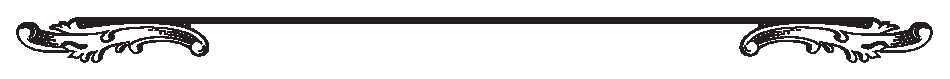
\includegraphics[width=1.06\textwidth,height=7.59mm]{hayamiz/images/chapter-title-ornament.eps}\vskip-7.59mm\vskip-0.5\Cvs
    \end{center}
    \par\nobreak
    \vskip 1\Cvs}} % 欧文は40pt
\def\@makeschapterhead#1{%
  {\parindent \z@ \raggedright
    \normalfont
    \interlinepenalty\@M
	\begin{center}
    {\LARGE \headfont #1}\par\nobreak\noindent
\hskip-0.03\textwidth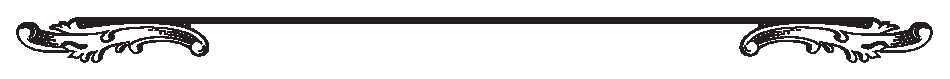
\includegraphics[width=1.06\textwidth,height=7.59mm]{hayamiz/images/chapter-title-ornament.eps}\vskip-7.59mm\vskip-0.5\Cvs
    \end{center}
	\par\nobreak
    \vskip 3\Cvs}} % 欧文は40pt
\makeatother

\renewcommand{\prechaptername}{}
\renewcommand{\postchaptername}{}

\makeatletter
\renewcommand{\thesection}{\S\,\@arabic\c@section}
\makeatother

\ifx\Cht\undefined
 \newdimen\Cht\newdimen\Cdp
 \setbox0\hbox{\char\jis2121}\Cht=\ht0\Cdp=\dp0\fi
\makeatletter
\long\def\linespace#1#2{\par\noindent
  \dimen@=\baselineskip\multiply\dimen@ #1\advance\dimen@-\baselineskip
  \advance\dimen@-\Cht\advance\dimen@\Cdp
  \setbox0\vbox{\noindent #2}\advance\dimen@\ht0\advance\dimen@-\dp0%
  \vtop to\z@{\hbox{\vrule width\z@ height\Cht depth\z@
   \raise-.5\dimen@\hbox{\box0}}\vss}%
  \dimen@=\baselineskip\multiply\dimen@ #1\advance\dimen@-\baselineskip
  \vskip\dimen@}
\makeatother

\title{Database Times Vol. 1}
\date{2012/8/11}
\author{Hotchpotch Society}

\begin{document}

\thispagestyle{empty}

\frontmatter

% タイトルページ
\begin{center}
 
\includegraphics[width=12cm]{hayamiz/images/title.eps}
 \par\vspace*{50mm}
 \noindent Hotchpotch Society
\end{center}

% まえがきページ
% -*- coding: utf-8 -*-

\chapter*{まえがき}
\addcontentsline{toc}{chapter}{まえがき}
\thispagestyle{plainhead}

The Database Times vol.1 をお手にとっていただきありがとうございます。

本書は、データベースシステムを中心として、様々な情報技術に関する話題を読
者の皆様にお届けすることを目的としています。みなさんは「データベースシス
テム」というものにどのようなイメージをお持ちでしょうか。SQLを投げるとデー
タを返してくれる、なんだかよくわからないけれど枯れた時代遅れの技術だとい
うイメージを持っている人が多いのではないかと思います。

しかしながら、実際のデータベースシステムは古の技術を土台として、その時代
の最先端の技術が詰め込まれた非常に魅力的な技術の集大成なのです。世界中で
生み出されるデータ量がどのくらいかご存知でしょうか。2010年までに生み出さ
れたデータ量はなんと1,227ペタバイト。しかも、2020年には7,910,000ペタバイ
トになるであろうと予測されています。人類が産み出そうとしているデータ量は、
まさに爆発的な勢いで増え続けています。このデータの膨張を支える縁の下の力
持ちがデータベースシステムです。加速するデータ量の増加に伴って、データベー
スも日々進歩を続けているのです。

そんなデータベースシステムがどのようにして生まれ、そして最近ではどんな
ことが話題になっているのか、本書を通してその一端に触れ、楽しんで頂ければ
幸いです。

\begin{flushright}
 2012年 8月

Hotchpotch Society
\end{flushright}

\newpage

\subsection*{お品書き}

\noindent {\bf ■ データベースシステムの夜明け}

今の世の中、データベースシステムといえばリレーショナルデータベースシステ
ムです。そのリレーショナルデータベースシステムが、一体どのようにして生み
出されたのか、そしてどのように発展を遂げていったのか、その歴史を辿ります。

\vspace*{\Cvs}

\noindent {\bf ■ PostgreSQLカンファレンス2012 レポート}

オープンソースDBMS代表格の一つであるPostgreSQLは、最近は業務でも用いられ
ることがかなり増えてきているようです。そんな PostgreSQL の最新技術事情に
触れられる PostgreSQL カンファレンスの参加レポートをお届けします。

\vspace*{\Cvs}

\noindent {\bf ■ とある世界で一番高速なBrainfuckインタプリタ}

近年ではSAP HANAやMemSQLなどの主記憶データベースが話題となっているように、
膨大するデータ量を捌ききるための「速さ」が強く求められています。データベー
スシステムはSQLというプログラミング言語の処理系という側面も持ちあわせてお
り、言語処理系の高速な実装はデータベースシステムには必要不可欠です。言語
処理系をいかに高速にするのか、その技術について世界最速Brainfuckインタプリ
タの実装者が解説します。

\vspace*{\Cvs}

\noindent {\bf ■ クラウド時代のDNS}

\noindent {\bf ■ IPv4がこの先生きのこるには}

最近では「クラウド」という言葉が話題となっていますが、その背景にはもはや
単一のコンピュータだけでシステムを構築してすべてがうまくいく時代は終焉を
迎え、ネットワークによりコンピュータを有機的に結合することが必須となりつ
つある現代の技術トレンドがよみとれます。ネットワーク技術では今一体何が起
きているのか、その最前線に迫ります。

\vspace*{\Cvs}

\noindent {\bf ■ 電算機技能者的同人誌執筆環境構築概論}

本書は \LaTeX で執筆されています。プログラマが \LaTeX で本を書くというの
はどういうことなのか、その開発(執筆)環境を紹介します。


\thispagestyle{plainhead}


% 目次ページ
\setcounter{tocdepth}{0} % show only chapters
\tableofcontents

\mainmatter

\pagestyle{fancy}

% 本文ここから
% -*- coding: utf-8 -*-

\chapter{PostgreSQLカンファレンス2012 レポート}

\begin{flushright}
 {\headfont はやみず}
\end{flushright}

2012年3月24日に日本PostgreSQLユーザ会主催で開催されたPostgreSQLカンファレ
ンス2012に参加してきました。この記事は、PostgreSQLカンファレンス全体の概
観についてレポートを記したものです。

このカンファレンスはオフィシャルサイトにあるように技術的な話題を中心とし
て、PostgreSQLに関する導入事例や技術的な話題を提供するためのカンファレン
スです。 昨年度の参加者約180名に対して今年度は275名(関係者含む)ということ
で、日本におけるPostgreSQLのユーザ層の広がりを感じさせます。 特にこの数年
はビジネスとしてこのカンファレンスに参加する方も増えているそうで、業務用
途としてのPostgreSQLの利用が広まっていることを示しているのではないかと思
われます。

Linuxの急速な普及をきっかけとして、今やオープンソースソフトウェアを業務に
おいて利用することは全く珍しくなくなっています。 PostgreSQLもその例に漏れ
ず、といったところでしょうか。本年度のカンファレンスのプログラムも、業務
用途におけるPostgreSQLの利用ということが一つの大きな軸として捉えられてい
るように見えます。 例えば、午後のプログラムは3トラック構成となっていたの
ですが、そのうちの1トラックは「マイグレーショントラック」と題して他の
DBMSからPostgreSQLへ移行することを主眼としたものであり、「商用 DB から
PostgreSQL への移行」「PostgreSQL がより使いやすく進化した Postgres Plus
Advanced Server の実力とは」などは明らかに商用DBを意識しています。また、
技術トラックやLightning Talkにおいて高可用・高性能なPostgreSQLクラスタに
関する発表がありました。業務用DBMSとしてはクラスタソリューションがほしい。
MySQLにはMySQL Clusterが、OracleにはOracle RACが、じゃあPostgreSQLはどう
なの?というポイントに答えを出すのが、今回のカンファレンスの一つの見所だっ
たのではないでしょうか。

もちろん、ビジネス的な側面だけではなく、技術の深い話もできるのがこのカン
ファレンスの魅力だと思います。午前中の基調講演では、PostgreSQLの大型移行
案件の事例紹介であるフランス社会保障機構の講演に加えて、PostgreSQLのコア
開発者でありコミュニティの中でも若手のエースと目されているEnterpriseDB社
のRobert Haas氏によるPostgreSQL 9.2の新機能に関する講演がありました。こち
らの講演では、メニーコア環境におけるスケーラビリティ向上の取り組みや、
Index-only Scanの導入、消費電力削減のための実装努力、レプリケーションの新
機能、その他細々とした新機能などが紹介されました。加えて、バージョン9.2よ
り後にどんな技術的な課題に取り組んでいくべきか、といった方向性についても
触れられていました。質疑応答も非常に活発に行われていたのが印象的です。一
つ残念だったのは、こちらの講演は発表・質疑応答ともに逐次翻訳が行われてい
たため、実際に話せる時間が半分になってしまっていたことです。英語のみで進
行してくれたほうが個人的には中身がもっと詰まって面白かったのではないかと
思いますが、難しいところですね。

もう1件技術的な講演として面白かったのは藤井雅雄氏、松尾隆利氏による
「PostgreSQL 9.1 同期レプリケーションと Pacemaker による高可用クラスタ化
の紹介」です。 こちらの発表では、まず藤井氏からPostgreSQLにおけるレプリケー
ションの詳細について紹介されていました。非同期レプリケーション、同期レプ
リケーションの動作や、何ができるのか、何ができないのかについて丁寧にまと
められており、レプリケーション機能の全体像を理解できる発表でした。またそ
れに加えて、9.2で導入される予定のレプリケーション関連の機能紹介や、周辺ツー
ルに関する紹介もありました。 その後、松尾氏により同期レプリケーション機能
とPacemakerを組み合わせることによる、障害発生時にもフェイルオーバ可能なク
ラスタ構成法についての発表が行われました。Pacemakerについては名前くらいし
か知らなかったのですが、障害発生からフェールオーバまでの流れがわかりやす
く図解されており、Pacemakerを知るという観点からも有用な発表であったように
思います。

本会議のほうについてはこんなところで、懇親会にも参加したのでの話をひとつ。
PostgreSQLのお役立ち情報源として参照している人も多いかと思われるLet's
Postgresという読み物サイトがあるのですが、こちらの運営をしている方とお話
をさせて頂きました。 この手の読み物サイトでは、最も需要の高い入門系記事や、
企業の提灯記事が並ぶというのがよくあるパターンなのですが、Let's Postgres
にはPostgreSQLの内部構造についてやたら詳しく書かれた記事がたくさんあり、
これは一体どういったことだろうと思っていたのでした。 そのことを聞いてみた
ところ、内部構造の多くは記事PostgreSQL本体にコミットしている開発者の方々
が好きで寄稿しているということだそうです。PostgreSQL自体が内部構造まで含
めた子細なドキュメントが充実していますが、新機能の実装詳解がこれほどまで
精力的に行われているソフトウェアはなかなかないのではないかとおもいます。
これらの記事は目的別ガイド:内部解析編としてまとめられています。内部の詳
解に加えて、開発プロセスへの参加方法についても紹介されており、非常に充実
した内容となっています。PostgreSQLの中身に興味がある人は必見ですね。

以上、簡単ではありますが参加レポートでした。

% TODO: もっと書く

% -*- coding: utf-8 -*-

\chapter{最近のデータベースシステム関係の話}
% * (アスタリスク)付きの \chapter* コマンドは原則不可とする

\begin{flushright}
 はやみず
\end{flushright}

この記事では、最近のデータベースシステムに関連する新しい話題を取り上げな
がら、その周辺の技術に関して思うことをだらだらと書き連ねてゆきます。あま
りまとまりがありませんが悪しからず。

\section{NoSQL}

流行りも一段落した感がありますが、まずはNoSQLの話から始めましょう。

NoSQLという言葉の定義自体が曖昧ではあるのですが、Not Only SQLを略して
NoSQL、つまり従前のSQLを使ったデータベースシステムではなく、それ以外の色々
なデータベース関連ソフトウェアのことを指します。

データベース分野においては、歴史的には``One size fits all''というスローガ
ンで語られることが多いのですが、RDBMSで全部やりましょうという時代が続いて
きました。ところが、データの量が増え、Webやモバイル端末の普及に伴ってユー
ザが増え、RDBMSでは対応しきれない場面が徐々に増えてきます。データベースの
大御所 Michael Stonebraker が2005年に ``One size fits all'' はもはや現実
的に無理が出てきているので、特定用途ごとに専用のデータベースエンジンを作っ
ていく必要がある、ということを指摘します。その動きとしてカラム志向型デー
タベースシステム、主記憶データベースシステムなどがあり、そのうちの一つに
NoSQLを位置づけることができるかと思います。



NoSQLという呼び方が非常に紛らわしいのですが、NoSQLと呼ばれている MongoDB、
CouchDB、Cassandra、Redis、memcached等々のソフトウェアと、従前のSQLベース
のデータベースシステムは直接対比して語るべきではない、というところに注意
が必要です。それどころか、NoSQLとひとくくりにされている諸々のソフトウェア
たちも、それぞれが同列に語られるべきものではありません。「これからの自体
SQLではなくNoSQLだ!」とか言っていると、「食べログなんてもう時代遅れ、時
代は塩スイーツ!」みたいに意味のわからない人になってしまうので注意しましょ
う\footnote{一方で、SQLとNoSQLが同列に語られることが多いのは、おそらく両
者を混同してほしいと思っている人たちがいるのではないかと思います}。

\section{Hadoop}

Hadoop、流行ってますね。

2004年にGoogleがMapReduceを発表し、

\section{はじめに}

\lettrine{ハ}
チロク世代がTwitter上で大々的に追悼されたのは記憶に新しい\footnote{「ハチロク世代追悼」で検索されたし}。かつてはIT業界を変えると期待されていた若者たちは、あるものは就職し、あるものは結婚し、そしてまたあるものは子供を持ち、別段IT業界を変えるでもなく普通のおっさんになろうとしている。もはやハチロク世代はアラサーであり、女子高生からはおっさんと呼ばれる年齢になってしまったのである。



% -*- coding: utf-8 -*-

\cleardoublepage
\plainifnotempty

\chapter{データベースシステムの夜明け}

\begin{flushright}
はやみず
\end{flushright}

\lettrine{デ}ータベースシステム無しでは、今日の社会は成り立たないと言って
良いでしょう。社会が高度に情報化された現在、世界中で大量のデジタルデータ
が日々生み出され、飛び交い、消費され、そして蓄積されてゆきます。2011年に
人類の生み出したデータ量は1,800ペタバイトにのぼります。一方で、膨大なデジ
タルデータは、単に生み出され、蓄積されてゆくだけではただのゴミも同様です。
必要なときに必要なデータが取り出せるよう、適切に管理してゆかなければなり
ません。そのための根幹たる存在が、データベースシステムなのです。

みなさんが馴染みのあるであろう MySQL や PostgreSQL、あるいは Oracle といっ
たデータベースシステムは、正確には「リレーショナルデータベースシステム」
と呼ばれています。リレーショナルデータベースシステムの歴史を辿ると、その
起源はある一篇の論文に遡ることができます。

その論文こそが、Edgar F.  Coddにより1970年に発表された ``A Relational
Model of Data for Large Shared Data Banks'' です。この論文は、リレーショ
ナルデータベースの最も重要な基礎となる{\bf リレーショナルデータモデル}を
提唱したもので、いわばデータベースシステム分野における金字塔です。古典力
学を Newton が拓き、相対性理論を Einstein が拓いたとするならば、データベー
スにおける一大分野であるリレーショナルデータベースを拓いたのは間違いなく
Edgar Codd その人といって間違いないでしょう。

そして、Codd によりリレーショナルモデル提唱から数年の後に、UNIXで動作する
世界初のリレーショナルデータベースシステムの開発プロジェクトが立ち上がり
ます。Michael Stonebraker率いる{\bf INGRESプロジェクト}です。Coddにより確
立されたリレーショナルデータベースシステムの基礎理論を、実際に動くソフト
ウェアとして実現し、そしてそれを世に広めたのがINGRESなのです。

本稿では、Coddによるリレーショナルデータモデルの提唱から、INGRESプロジェ
クトの黎明期の記録を辿り、現代の社会を支えるデータベースシステムがいかに
して創り上げられたのか、その歴史を紐解いてみようと思います。

\section{リレーショナルデータモデルの登場}

1960年代以前のデータベースシステムは階層型データモデル、やネットワーク型
データモデルというデータモデルに基づいて構築されていました。

\begin{figure}[tb]
 \begin{minipage}{0.48\textwidth}
  \begin{center}
   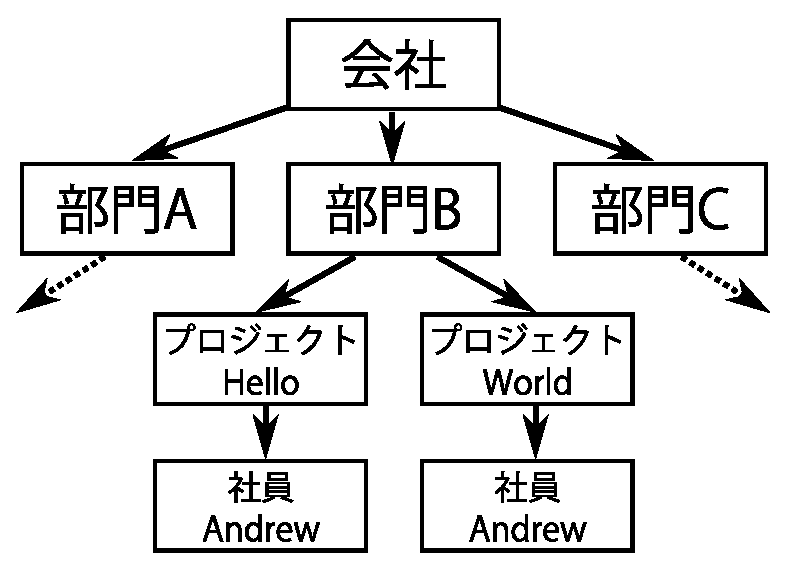
\includegraphics[width=5cm]{hayamiz/images/hierarchical-data-model.eps}
   \caption{階層型データモデル}
   \label{214539_12Jul12}
  \end{center}
 \end{minipage}
 \begin{minipage}{0.48\textwidth}
  \begin{center}
   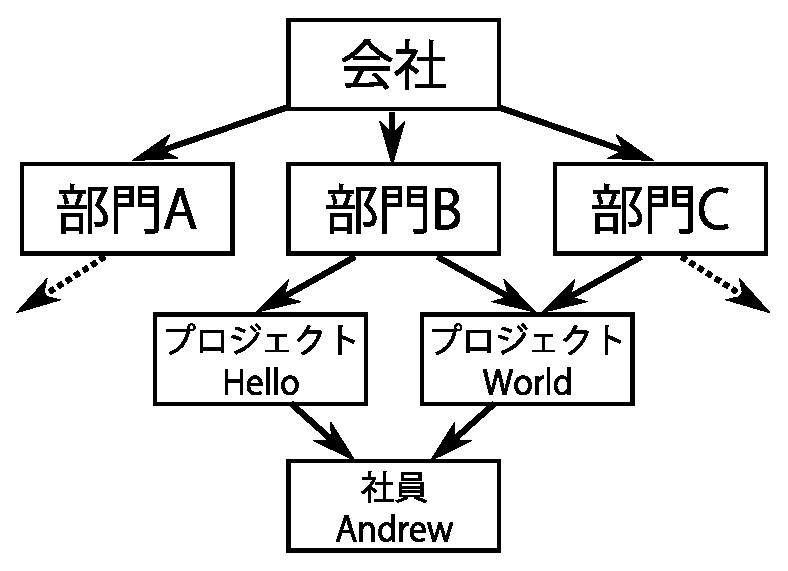
\includegraphics[width=5cm]{hayamiz/images/network-data-model.eps}
   \caption{ネットワーク型データモデル}
   \label{214707_12Jul12}
  \end{center}
 \end{minipage}
\end{figure}

階層型データモデルというのは、木構造を用いてデータを組織化したデータモデ
ルです。たとえば会社組織を階層型データモデルで表そうと思うと、会社の下に
は複数の部門が属しており、各部門の下には複数のプロジェクトがあり、各プロ
ジェクトの下には社員が属している、というようにスキーマを定義してゆきます
(図\ref{214539_12Jul12})。ここで、例えば2つのプロジェクトHelloとWorldに属
する1人の社員Andrewがいたとしたらどうでしょう。階層型データモデルでは、あ
るデータの実体(ここでは1人の社員)は親となるデータの実体(プロジェクト)
を複数持つことができません。そのため、各プロジェクトごとにAndrewのデータ
を持つことになり、データの重複が生じてしまいます。また、部門Bと部門Cが共
同でプロジェクトWorldを運営していることを表現しようと思うと、プロジェクト
のデータに加えてその下にぶら下がっている社員のデータも併せてコピーしなけ
ればなりません。このような欠点を克服したのがネットワーク型データモデルで
す(図\ref{214707_12Jul12})。ネットワーク型データモデルでは、データの実
体が複数の親を持つことができる有向グラフをデータ構造として採用したため、
前述のようなデータ重複の問題は発生しません。

ネットワーク型モデルによりより一般的なデータ構造を表現できるようにはなり
ました。しかし、階層型モデルやネットワーク型モデルに基づくデータベースは、
データのアクセスに一つ大きな問題を抱えていました。これらのデータベースに
おいてデータの問い合わせを行う際には、データの構造がどのようになっている
かを把握し、そしてどのような手順でデータを取得するかを利用者が知っている
必要があったのです。例えば図\ref{214707_12Jul12}のデータベースにおいて社
員Andrewのデータを取得するためには、「会社のデータを読みとり、部門Bのデー
タを読み取り、プロジェクトHelloのデータを読み取り、社員Andrewのデータを読
み取る」という手順を指定してあげなければなりません。このように、欲しいデー
タにアクセスするための``how'' をもって問い合わせを行うデータベースシステ
ムは、ユーザがデータの案内(navigation)をするという意味で{\bf ナビゲーショ
ナルデータベースシステム}と呼ばれます。

もしもナビゲーショナルデータベースシステムにおいて、図
\ref{214707_12Jul12}の会社で組織改変があり、各部門の下には課が設置され、
その下にプロジェクトが属するという構造にデータベースが修正されたとしたら
どうなるでしょう。これまで社員のデータにアクセスするアプリケーションは会
社→部門→プロジェクト→社員とたどっていましたが、会社→部門→課→プロジェ
クト→社員とたどるように修正しなければなりません。このように、ナビゲーショ
ナルデータベースシステムでは、ある特定のデータのみに興味があったとしても、
その上位構造に変化があった時にはデータにアクセスする方法を再構成しなけれ
ばなりませんでした。当時IBMはIMSという階層型データモデルにもとづくデータ
ベースシステムを開発していましたが、IMSを使ったシステムではデータ構造の変
更に伴うコードのメンテナンスにほとんどの時間を吸い取られていました。

歴史的には、階層型モデルはそのシンプルさ故に初期のデータベースシステムに
おいて採用され、その後により一般的なデータの組織化を行うことができるよう、
ネットワーク型モデルが発明されます。1969年にはCODASYLという委員会によって、
ネットワーク型データモデルの標準化が行われ、データベースシステムの情勢は
階層型モデルからネットワーク型モデルに移るかと思われました。

そこに登場したのが、1970年\footnote{正確にはリレーショナルデータモデルの
論文は1969年にIBMの社内技術報に掲載され、翌1970年に米国コンピュータ学会の
論文誌に掲載されます。}にCoddによって提唱されたリレーショナルデータモデル
です。リレーショナルデータモデルでは、データの論理的な構造と物理的な構造
が独立しているため、データ構造を変更するたびにアプリケーションを書き直す
必要がありません。また、ユーザは「どんなデータが欲しいか」を記述するたけ
で、具体的なアクセス方法はデータベース側が判断してデータを取得することが
できます。つまり、ナビゲーショナルデータベースシステムでは ``how'' を与え
なければデータのアクセスが行えなかったのですが、リレーショナルデータベー
スは ``what'' を与えるだけでデータのアクセスが可能となります\footnote{リ
レーショナルモデルの数学的な定義や、なぜそれにより``what''でデータの問い
合わせが可能となるのかの説明については、それだけで一冊の本になってしまう
ので他書に譲ります。}。

また、リレーショナルモデルは集合論にもとづくしっかりとした数学的基礎の上
に成り立っており、後のデータベースシステム研究の大きな基盤となりました。
これまでプログラマによるある種の職人芸の上に成り立っていたデータベースシ
ステムは、リレーショナルデータモデルの登場によって科学の領域へと押し上げ
られたのです。

\section{INGRESプロジェクト始動}

リレーショナルデータモデルがCoddによって提唱されてから3年が経った1973年が
終わろうとする頃、その論文が一人の若き研究者の目に留まりました。その人こ
そ、INGRESプロジェクト、そして後のデータベース業界全体を率いる存在となる
Michael Stonebraker です。1971年にミシガン大学で博士号を取得し、UC
Berkeleyで研究職についたばかりのStonebraker はテニュアトラック
\footnote{テニュアとは大学における終身雇用資格のことです。若手研究者は任
期の限られた研究職につき、テニュア獲得を目指して研究業績を積み上げてゆく、
というの米国における一般的な研究者のキャリアパスです。このテニュア獲得の
ための若手研究者が通る道をテニュアトラックと呼びます。テニュアトラックで
いかに論文を``量産''できる研究ネタを選ぶかというのは、若手研究者にとって
は人生に関わる重要な決断なのです。}を走り始めたばかりであり、何か良い研究
のネタはないかと思案していたところでした。そんな Stonebraker にとって、リ
レーショナルモデルは恰好の研究対象だったのでしょう\footnote{ちなみに
Stonebraker の博士論文は ``The Reduction of Large Scale Markov Models
for Random Chains'' というタイトルで、もともとは数学寄りの研究をしていた
ようです。 }。リレーショナルデータモデルに出会った Stonebraker は、
Eugene Wong と共にリレーショナルデータベースシステムの実装に乗り出します。
こうしてINGRESプロジェクトは始まりました。

% http://genealogy.math.ndsu.nodak.edu/id.php?id=31091

INGRESという名前は、{\bf IN}teractive {\bf G}raphic and {\bf RE}trieval
{\bf S}ystem の頭文字をとったもので、本来は UC Berkeley の経済学の研究チー
ムのために、地理情報をグラフィカルに表示するためのシステム研究として予算
を獲得していたプロジェクトでした。そこは本音と建前で、まずはデータを効率
的に取得するためのデータベースシステムが必要だ、ということで Stonebraker
達はデータベースシステムの開発にのめりこんでゆきます。

こうして走り始めたINGRESプロジェクトですが、データベースシステムを動かす
ためのコンピュータはありませんし、そもそも Stonebraker や Wong は大きなプ
ログラム開発の経験すらありませんでした。リレーショナルデータベースシステ
ムの先駆けであるINGRESは、まさにゼロからのスタートでした。

何はなくともデータベースシステムの開発環境がなければ話になりません。
INGRESプロジェクトが始まって Stonebraker が最初に取り組んだのは、コンピュー
タの調達と開発環境作りでした。当時といえば、データベースシステムを構築す
るためには高価なメインフレームを導入して、COBOLでプログラムを書くという時
代でした。リレーショナルデータベースシステムのように、まだ世の中に存在す
らしていないソフトウェアのために、研究職になりたての Stonebraker がメイン
フレームを手に入れることができるわけもありません。

そんな中、ミニコンピュータと呼ばれる、いわゆる現在のPCの先駆けとなる安価
なコンピュータシステムが1960年代に生まれ、そして1970年代にはミニコンピュー
タをビジネスに活用しようという動きが高まり、小型ビジネスコンピュータ市場
が生まれました。時を同じくして、ベル研究所では Ken Thompson 達によってミ
ニコンピュータ上で動作する汎用オペレーティングシステムUNIXの開発プロジェ
クトが始まりました。UNIXはもともとアセンブリで実装されていましたが、
Dennis Ritchie 達によってUNIX開発のためにC言語が開発され、1973年にはC言語
に移植されました。そう、まさにINGRESプロジェクトが始まったその年です。

Stonebraker は開発環境として UNIX を、そしてINGRESの実装言語としてC言語を
使うことを決めます。そして UNIX が動作するコンピュータとして選ばれたのが、
DECのPDP-11/70でした。UNIXが最初にベル研究所以外の場所でインストールされ
たのがこのINGRESプロジェクトであり、インストール時には Ken Thompson と
Dennis Ritchie が5MBのディスクを抱えてやってきたそうです。

\section{INGRESの進化}

INGRESプロジェクトでは、リレーショナルデータベースシステムの実装における
重要な技術が多数生み出されてゆきました。当時のINGRESがどのように設計され
ていたのか、1976年に発表された論文``The design and implementation of
INGRES''をもとに、その技術的な側面を概観してゆきます。

\begin{center}
 \begin{minipage}{0.95\textwidth}
  \begin{screen}
   以降の説明で使われる用語

   \footnotesize
   \term{リレーション}{リレーショナルデータモデルにおける、いわゆ
   るテーブルのこと}

   \term{タプル}{リレーショナルデータモデルにおける、いわゆるレコードの
   こと}

  \end{screen}
 \end{minipage}
\end{center}

\subsection{クエリ言語QUELとEQUEL}

リレーショナルデータベースでは、それ以前のナビゲーショナルデータベースと
は異なり、どんなデータが欲しいか``what''を記述するだけで、具体的にどのよ
うなデータ構造やアルゴリズムが実装されているかを一切知る必要なくデータを
取得することができる、というのが大きなウリの一つです。その``what''を記述
するための言語がクエリ言語です。皆さんのよく知っているSQLもクエリ言語の一
つです。

INGRESプロジェクトでは、クエリ言語としてQUELが開発されます。リレーショナ
ルデータモデルに併せて Codd はDSL/APLHAというクエリ言語を1971年に発表して
いるのですが、DSL/ALPHAは数学的な表記\footnote{DSL/ALPHAは関係演算
(relational calculus)をベースとして、量化子$\exists, \forall$や、論理演算
の記号$\lnot,\land,\lor$などがほぼそのまま用いられいていました}に基づいて
おりやや一般的にわかりやすいものではありませんでした。QUELはDSL/ALPHAをベー
スとして、数学的な表記のない``やさしい''クエリ言語として設計されました。

QUELがどんな言語なのか、簡単なサンプルコード\footnote{1975年のINGRESの論
文より引用}をみてみましょう。

\begin{center}
 \begin{minipage}{0.9\textwidth}
  \begin{verbatim}
RANGE OF C IS CITY
RETRIEVE INTO W(C.CNAME,
                DENSITY = C.POPULATION / C.AREA)
         WHERE C.STATE = 'California'
           AND C.POPULATION > 50000
  \end{verbatim}
 \end{minipage}
\end{center}

このサンプルコードでは、カリフォルニア州にある人口5万人以上の市について、
市の名前と人口密度の一覧を取得するという処理を行っています。一行目の
RANGE文では、処理の対象としてCITYリレーションを選択して、CITYリレーション
のタプルを表す変数名Cを宣言しています。二行目のRETRIEVE文は、SQLでいうと
ころのSELECT文に相当します。処理の結果は、一時テーブルとして作成されるWに
保存されます。細かい表記の違いを別にすると、現在使われているSQLとそれほど
大きな違いがないことがわかると思います。

\subsection{アクセスメソッドとデータ構造}

アクセスメソッドとは、その名前の通りデータベースに保存されているデータに
アクセスするための方法です。例えば、とある会社の従業員のデータがEMPリレー
ションに1万人分保存されていたとします。この中から、ある従業員1人分のタプ
ルを取り出すには、どうすればよいでしょうか。もっともナイーブには、EMPリレー
ションを頭から全部スキャンして、目的の従業員のタプルを探すという方法が考
えられます。これも立派なアクセスメソッドの一つですが、1人分のデータを探す
にはちょっと効率が悪すぎます。従業員番号でタプルを並べておいて、二分探索
するというやり方も簡単に思いつく方法です。これもアクセスメソッドの一つと
いえます。

アクセスメソッドには様々な実装方法があり、それぞれが得意とするデータアク
セス、苦手とするデータアクセスのパターンがあります。データベースシステム
のように総合的なデータの管理を行うためのシステムでは、複数のアクセスメソッ
ドを利用できる必要があります。

\subsubsection{アクセスメソッドインターフェース}

INGRESには、複数のアクセスメソッドを利用するためのインターフェースが
定められています。INGRESで標準的に提供されるアクセスメソッドはすべてこの
インターフェースを介して提供されており、またこのインターフェースに従って
実装することで独自のアクセスメソッドを追加することができるように設計され
ています。

INGRESで定められているアクセスメソッドインターフェースは次の通りです:
\begin{enumerate}
 \item {\bf OPENR}({\it descriptor}, {\it mode}, {\it relation\_name})
 \item {\bf GET}({\it descriptor}, {\it tid}, {\it limit\_tid}, {\it
       tuple}, {\it next\_flag})
 \item {\bf FIND}({\it descriptor}, {\it key}, {\it tid}, {\it key\_type})
 \item {\bf PARAMD}({\it descriptor}, {\it access\_characteristics\_structure})
 \item {\bf PARAMI}({\it index\_descriptor}, {\it access\_characteristics\_structure})
 \item {\bf INSERT}({\it descriptor}, {\it tuple})
 \item {\bf REPLACE}({\it descriptor}, {\it tid}, {\it new\_tuple})
 \item {\bf DELETE}({\it descriptor}, {\it tid})
 \item {\bf CLOSER}({\it descriptor})
\end{enumerate}
{\bf OPENR} と {\bf CLOSER} はプログラマにとってはファイル操作等でお馴染
みの関数でしょう。{\bf OPENR} で指定したリレーションを開き、リレーション
のディスクリプタを取得します。以降、このリレーションに対するアクセスはこ
のディスクリプタを以って行われます。一連のアクセスが完了した後は、{\bf
CLOSER} によってリレーションを閉じます。

{\bf GET} は、タプルID(tid)をキーとしてタプルのデータを取得するための関数
です。{\it tid}でタプルIDの下限を、{\it limit\_tid}でタプルIDの上限を指定
することができ、{\bf GET}が呼び出されるとこの条件にマッチする最初のタプル
を見つけてきて、そのデータを {\it tuple} に書き込みます。また、{\it
next\_flag}にTRUEを指定して{\bf GET}を呼び出した場合には、次にマッチする
タプルのIDを{\it tid}に書きこむため、連続してタプルを読みだしてゆくことが
できます。

{\bf FIND}は、{\it key}で指定した検索キーにマッチするタプルIDを取得するた
めの関数です。{\it key\_type}で完全一致検索、範囲検索などの検索モードを指
定することができます。

{\bf PARAMD}、{\bf PARAMI}は{\bf FIND}において利用可能な検索キーの種類や、
検索モードを調べるための関数です。それぞれ、データファイル用と、索引ファ
イル用に利用されます。

{\bf INSERT}はタプルを挿入するための関数、{\bf REPLACE}は既に存在するタプ
ルを更新するための関数、{\bf DELETE}はタプルを削除するための関数です。

\subsubsection{データ構造}

INGRESでは、{\bf ヒープ}、{\bf ハッシュ}、{\bf ISAM}、{\bf 圧縮ハッシュ}、
{\bf 圧縮ISAM}の5種類のアクセスメソッドが提供されています。

{\bf ヒープ}は単純にタプルを並べてゆくだけの最も単純な構造で、タプルを探すとき
は毎回線形探索を行います。非常にタプル数の少ないリレーションや、クエリの
実行結果を格納する一時的なリレーションに適しています。

\begin{figure}[tb]
 \begin{center}
  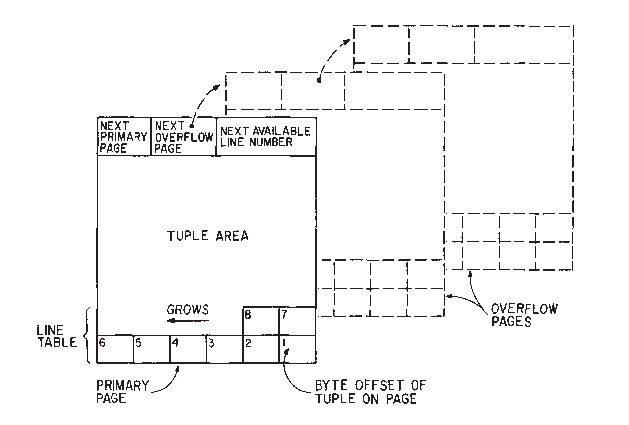
\includegraphics[height=66mm]{hayamiz/images/page-layout-ingres.eps}
  \caption{INGRESのページ構造}
  \label{174456_16Jul12}
 \end{center}
\end{figure}

{\bf ハッシュ}と{\bf ISAM}は、検索キーを用いて少量のタプルに対するアクセ
スを高速に行うことを可能とする構造です。{\bf ハッシュ}はハッシュテーブル
を使って、{\bf ISAM}は探索木を使って、検索キーとタプルIDの関連付けを行う
ことで、高速なアクセスを実現しています。INGRESでは、タプルIDは (ページ番
号, ページ内ライン番号) という値のペアによって表現されているので、タプル
IDさえわかれば目的のデータの在り処がわかります。

ページの構造は図\ref{174456_16Jul12}のようになっています。ページの先頭に
はヘッダ情報があり、またページの末尾にはラインテーブルと呼ばれるデータが
格納されています。ラインテーブルの各要素は、タプルのデータがページ内のど
の位置にあるかのオフセット情報を保持しています。タプルIDに含まれているペー
ジ内ライン番号は、このラインテーブル内のインデックス番号となっているので、
タプルIDさえわかればタプルのデータがどこにあるのかがわかるようになってい
ます。この構造には、タプルの物理的な位置が変化しても、ラインテーブルを更
新するだけで、タプルIDは変化することがないという利点があります。

\subsubsection{アクセスメソッドまとめ}

\begin{figure}
 \begin{center}
  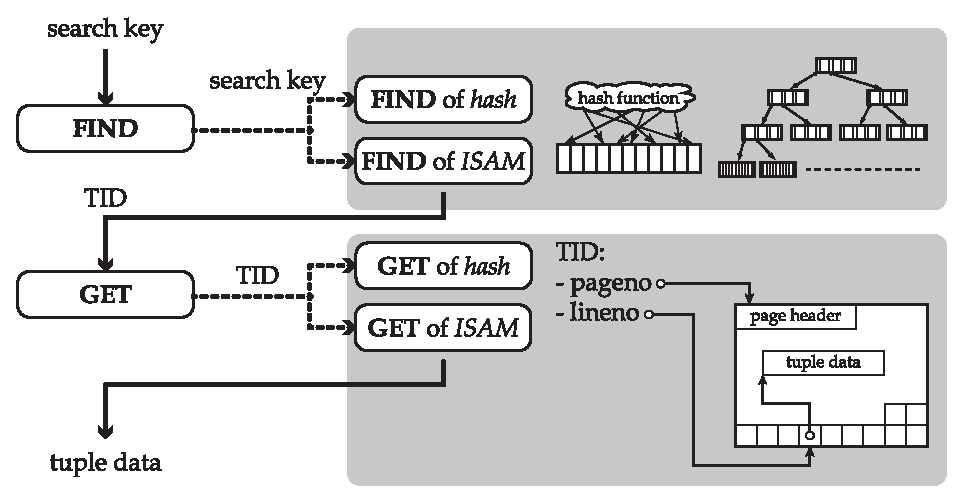
\includegraphics[width=100mm]{hayamiz/images/access-method.eps}
  \caption{検索キーを用いたアクセスメソッドによるタプルデータの取得}
  \label{190817_16Jul12}
 \end{center}
\end{figure}

検索キーが与えられてから、タプルのデータが得られるまでの一連の流れを図
\ref{190817_16Jul12}にまとめました。まずは検索キーが与えられると、{\bf
FIND}を呼び出してタプルIDを取得します。{\bf FIND}の中では、ハッシュテーブ
ルや木構造を用いて効率的にタプルIDの検索が行われます。そして、得られたタ
プルIDを引数として{\bf GET}を呼び出すことで、ページを読み出し、タプルのデー
タが取得されます。

この基本的なデータアクセスの枠組みは、INGRESの頃に確立され、現在でも殆ど
変わること無く引き継がれています。

ただ1980年頃まで、INGRESには B$^+$-tree を用いたアクセスメソッドは実装さ
れていませんでした。ISAMとB$^+$-treeはよく似ているのですが、根本的な違い
としてISAMは静的なアクセスメソッドであるのに対し、B$^+$-treeは動的なアク
セスメソッドであるということです。どちらも多分木構造を索引として用いてい
ますが、ISAMではデータの挿入や削除のたびに木構造を変更することはなく、適
当なタイミングでまとめて木構造を作り直します。そのため、頻繁にデータの挿
入、削除が行われる場合にはどんどん構造劣化が進み、アクセス性能が落ちてし
まいますが、参照が非常に多い場合には良い性能を発揮します。一方、
B$^+$-treeはデータの挿入、削除のたびに木構造を動的にバランスさせるために、
ISAMで起きるような構造劣化は起きません。しかし、1回の処理あたりのオーバー
ヘッドはISAMよりも大きくなってしまいます。

INGRESの開発において、何度もB$^+$-treeの導入が検討され、その度に採用が見
送られてきたようです。しかしながら、1980年のINGRES開発を振り返る論文にお
いて、StonebrakerはB$^+$-treeの採用を見送ってきたのは ``major mistakes''
の一つであり、次にアクセスメソッドを再検討する際にはB$^+$-treeも実装する
であろうと述べています。

また、INGRESのアクセスメソッドはUNIXのファイルシステムの上に構築されてい
たのですが、UNIXのファイルシステムによるオーバーヘッドが当初予測していた
よりも深刻なものであり、独自のファイルシステムを実装するべきであった、と
も同論文では述べられています。実際に、3年後に発表された論文において
Stonebraker 達は独自に実装したファイルシステムを使った場合と性能比較を行っ
ており、最大で70\%程度性能が向上することを確認しています。このように
INGRESの開発過程で得られた知見は、UNIXの開発にもフィードバックされ、その
発展にも大きく貢献しました。

\subsection{クエリ処理エンジン}

\section{System R}

INGRESプロジェクトからすこし遅れて、IBMでもリレーショナルデータベースシス
テム System R の研究開発が始まります。リレーショナルデータモデルの父であ
る Codd はIBMで働いていたにも関わらず、歴史を振り返るとIBMはリレーショナ
ルデータベースシステム開発において常に後塵を拝しています。

TODO:

\section{エピローグ}

1970年代には、Coddによるリレーショナルデータモデルの提唱に始まり、INGRES
やSystem Rの研究によってリレーショナルデータベースシステムが実用に耐えう
るものであることが証明されました。1981年には、Coddはその功績が認められ計
算機科学分野において最も権威ある賞であるチューリング賞を受賞します。

そして1970年代の終盤から1980年代は、商用リレーショナルデータベースシステ
ムが次々と登場し、熾烈な戦いを繰り広げてゆきます。

1977年、現在の Oracle の前身である Software Development Laboratories が
Larry Ellison と Robert Miner によって設立され、1979年にはSQLベースの商用
リレーショナルデータベースシステムとしては世界初となる Oracle RDBMS の発
売を開始します。

1979年、Jack Shemer、Philip Neches、Walter Muir、Jerold Modes、William
Worth、Carroll ReedによってTeradataが設立され、1984年には世界初の並列デー
タベースシステムDBC 1012をリリースします。

1980年、Lawrence Rowe、Michael Stonebraker、Eugene Wong、Gary
Morgenthaler によって INGRES 商用化のために Relational Technology (後の
Ingres Corp.)が設立され、翌1981年に最初の商用INGRESをリリースします。

時を同じくして、Roger Sippl と Laura King によって 1980年に Relational
Database Systems (後の Informix Software) が設立され、翌1981年に
Informix がリリースされます。

IBMは1981年にSQL/DSを、さらに1983年にはDB2をリリースしてリレーショナルデー
タベース市場に乗り出します。エンタープライズ市場の覇者であるIBMのこの動き
は、旧来のナビゲーショナルデータベースシステムに対する新興勢力リレーショ
ナルデータベースシステムの勝利を決定的なものにします。

1984年、Mark Hoffman、Bob Epstein、Jane Doughty、Tom Hagginによって
Sybaseが設立され、1986年にリレーショナルデータベースシステムSybaseをリリー
スします。後にSybaseはMicrosoftと提携してSybase SQL Serverを開発し、その
設計はMicrosoft SQL Serverにも受け継がれています。

同1984年、ミニコンピュータ市場を牽引するDECがOpenVMSオペレーティングシス
テムにおける機能として DEC Rdb を発表します。

1986年、無停止コンピュータシステムを主な事業として手がける Tandem
Computers が NonStop SQL をリリースします。

そして1990年代には更にプレイヤーが増えつつもその統廃合が進み、オブジェク
ト指向データベースシステムなど進行技術の登場、オープンソースのデータベー
スシステム隆盛の兆候など、データベースシステムは新たな時代へと突入してゆ
きます。

\section*{参考文献}

\small

\begin{itemize}
 \item E. F. Codd, ``A Relational Model of Data for Large Shared Data
       Banks'', {\it Communications of the ACM}, Volume 13, Number 6,
       1970
 \item E. F. Codd, ``A data base sublanguage founded on the relational
       calculus'', {\it Proceedings of the 1971 ACM SIGFIDET workshop
       on Data Description, Access and Control}, 1971
 \item C. J. Date, E. F. Codd, ``The relational and network approaches: Comparison of the
       application programming interfaces'', {\it Proceedings of the
       1974 ACM SIGFIDET workshop on Data Description, Access and
       Control}, 1975
 \item G. Held, M. Stonebraker, E. Wong, ``INGRES--A relational data
       base management system'', {\it Proceedings of AFIPS 1975 NCC},
       Volume 44, 1975
 \item M. Stonebraker, G. Held, E. Wong, P. Kreps, ``The design and
       implementation of INGRES'', {\it ACM Transactions on Database
       Systems}, Volume 1, Issue 3, 1976
 \item G. Held, M. Stonebraker, ``B-trees re-examined'', {\it Communications of the
       ACM}, Volume 21, Issue 2, 1978
 \item M. Stonebraker, ``Retrospection on a database system'', {\it ACM
       Transactions on Database Systems}, Volume 5, Issue 2, 1980
 \item D. Chamberlin, M. Astrahan, M. Blasgen, J. Gray, W. F. King,
       B. Lindsay, R. Lorie, J. Mehl, T. Price, F. Putzolu, P. Selinger,
       M. Schkolnick, D. Slutz, I. Traiger, B. Wade, R. Yost, ``A
       history and evaluation of System R'', {\it Communications of the
       ACM}, Volume 24, Issue 10, 1981
 \item M. Stonebraker, J. Woodfill, J. Ranstrom, M. Murphy, M. Meyer,
       E. Allman, ``Performance enhancements to a relational database
       system'', {\it ACM Transactions on Database Systems}, Volume 8,
       Issue 2, 1983
 \item Relational Technology Inc., ``INGRES The Distributed SQL
       Relational Database System Press Kit'', 1987
 \item National Research Council, ``Funding a Revolution: Government
       Support for Computing Research'', Natl Academy Pr, 1999
 \item M. Stonebraker, J. M. Hellerstein, ``What Goes Around Comes
       Around'', {\it Readings in Database Systems, Fourth Edition},
       Morgan Kaufmann, 2005
 \item A. Ances, ``RDBMS Workshop: Ingres and Sybase'', Computer
       History Museum, 2007
\end{itemize}

and so many online resources

\normalsize

% -*- coding: utf-8 -*-
%!TEX root = ../book.tex

%\cleardoublepage
%\plainifnotempty

\chapter{とある世界で一番高速なBrainfuckインタプリタ}
\begin{flushright}
hogelog
\end{flushright}

\section{まえがき}
\lettrine{世}
の中にはたくさんのプログラミング言語が存在します。
Dennis RitchieはUnixを記述するためにC言語を作り
\footnote{The Development of the C Language* 
\verb|http://cm.bell-labs.com/cm/cs/who/dmr/chist.html|
},
Tecgrafチームはブラジルの貿易障壁の影響下で
Luaを
\footnote{
The Evolution of Lua
\verb|http://www.lua.org/doc/hopl.pdf|
},
そしてUrban M\"ullerは
チューリング完全な最小限の言語として
Brainfuckを作成しました
\footnote{
\verb|http://www.muppetlabs.com/~breadbox/bf/|
}
。

世の中にはたくさんのプログラミング言語処理系が存在します。
例えばRuby言語には
まつもとゆきひろによるオリジナル実装を元にした
MRI\footnote{
\verb|http://www.ruby-lang.org/ja/|
},
JVM上で動作する
JRuby\footnote{
\verb|http://jruby.org/|
},
JITコンパイラや世代別GCなどが組み込まれた
Rubinius\footnote{
\verb|http://rubini.us/|
},
組み込みスクリプトエンジン向けとして作られた
mruby\footnote{
\verb|https://github.com/mruby/mruby/|
}
など様々な処理系があります。
例えば大規模分散処理のためHadoopフレームワークを利用したければ
JRubyを使うこともあるでしょう。
エディタアプリケーションにスクリプト機能を組み込むためにはmrubyを
使うかもしれません。
言語処理系にとって重要な機能は
使う局面によって変わってきますが,
処理系が高速であればだいたいの人は嬉しいでしょう?

Brainfuckという言語は
\verb|+ - > < , . [ ]|
という8個の命令しか存在しない,
処理系の実装が容易な言語です
\footnote{
\verb|http://www.kmonos.net/alang/etc/brainfuck.php|
とかわかりやすい解説だと思います
}。
以下ではBrainfuckインタプリタの高速化を通じて
\textbf{インタプリタの高速化}
技術について親しんでいきましょう。
とりあえずはこの記事のタイトル通りに
{\Large \textbf{世界で一番高速なBrainfuck処理系}}
を作ってみましょう。

なお以下で示すサンプルコードは
筆者のgithubリポジトリ
\footnote{\verb|https://github.com/hogelog/sample-code/tree/master/dbtimes-vol01|}
から適宜参照できます。

\section{普通の処理系}
{\scriptsize
\verb|https://github.com/hogelog/sample-code/blob/master/dbtimes-vol01/bf.cpp|
}

さて,まずはなんの高速化も施されていない
Brainfuck処理系を実装します。
(図\ref{bf.cpp})

たったこれだけの記述で一応ちゃんとした
言語処理系になるんだから楽で良いですね。

\begin{figure}[hbt]
\begin{minipage}{0.5\hsize}
{\scriptsize
\begin{verbatim}
#include <stdio.h>
#include <string>
int main() {
  std::string code;
  for (int ch;(ch=getchar())!=EOF;)
    code.push_back(ch);
  static int membuf[30000];
  int *mem = membuf;
  int depth = 0;
  for (size_t pc=0;pc<code.size();++pc) {
    switch(code[pc]) {
      case '+': ++*mem; break;
      case '-': --*mem; break;
      case '>': ++mem; break;
      case '<': --mem; break;
      case ',': *mem = getchar(); break;
      case '.': putchar(*mem); break;
      case '[':
\end{verbatim}
}
\end{minipage}
\begin{minipage}{0.5\hsize}
{\scriptsize
\begin{verbatim}
        if (*mem == 0) {
          depth = 1;
          while (depth != 0) {
            switch(code[++pc]) {
              case '[': ++depth; break;
              case ']': --depth; break;
            }}}
        break;
      case ']':
        depth = -1;
        while (depth != 0) {
          switch(code[--pc]) {
            case '[': ++depth; break;
            case ']': --depth; break;
          }}
        --pc;
        break;
    }}
  return 0;
}
\end{verbatim}
}
\end{minipage}
\caption{
普通のBrainfuckインタプリタ
}
\label{bf.cpp}
\end{figure}

\section{インタプリタ高速化}
上述したインタプリタは簡潔ですしちゃんと動くので良いのですが
あまり高速ではないので,
いくつかの高速化を施して世界最速インタプリタにしてみましょう。

\subsection{VM化}
{\scriptsize
\verb|https://github.com/hogelog/sample-code/blob/master/dbtimes-vol01/bf-vm.cpp|
}

プログラムの文字列を逐次解釈するインタプリタを
高速化する手法として,
プログラムをVM\footnote{Virtual Machineの略}
命令列へ変換する部分と
VM命令列のインタプリタ部分に分ける方法がよく知られています。
RubyインタプリタのMRIは
バージョン1.9から
独自VMを内蔵するようになり,
大幅な高速化に成功しました。
ここではBrainfuckインタプリタの
VM化を試してみましょう。

図\ref{bf.cpp}
のプログラムは
\verb|[ ]|命令を処理する部分に
while文があるのが気になります。
\verb|[|
と対応する
\verb|]|
は一度調べればわかるのに,
毎回1文字ずつ探すのは効率がよくありません。
\verb|[ ]|命令
を対応するVM命令の位置を保持するVM命令へと
変換することで,
\verb|[ ]|命令
の処理部分から
while文が消えます。
(図\ref{bf-vm.cpp:loop})

またプログラムを実行するforループで毎回
\verb|pc<code.size()|
とチェックするのも無駄です。
処理するVM命令列の最後に
「処理を終了する」命令を一つ追加することで,
終了判定もswitch文の中に混ぜることができました。
(図\ref{bf-vm.cpp:finish})

\begin{figure}[hbt]
\begin{minipage}{0.3\hsize}
{\scriptsize
\begin{verbatim}
struct Instruction {
    char op;
    int jmp;
};
\end{verbatim}
}
\caption{
VM命令構造
}
\label{bf-vm.cpp:structure}
\end{minipage}
\begin{minipage}{0.3\hsize}
{\scriptsize
\begin{verbatim}
case '[':
    if (*mem == 0) {
        pc = code.jmp;
    }   
    break;
case ']':
    pc = code.jmp;
    break;
\end{verbatim}
}
\caption{
[]命令処理部分
}
\label{bf-vm.cpp:loop}
\end{minipage}
\begin{minipage}{0.3\hsize}
{\scriptsize
\begin{verbatim}
    for (size_t pc=0;;++pc) {
        Instruction code = codes[pc];
        switch(code.op) {
            ...
            case '\0':
                return;
\end{verbatim}
}
\caption{
終了処理
}
\label{bf-vm.cpp:finish}
\end{minipage}
\end{figure}


\subsubsection{direct threaded code}
{\scriptsize
\verb|https://github.com/hogelog/sample-code/blob/master/dbtimes-vol01/bf-vm2.cpp|
}

VMの高速化手法の一つに
direct threaded code
と呼ばれる手法があります。
詳細は
Ruby 1.9
のVM化を主導した
笹田耕一さんによる記事
YARV Maniacs
\footnote{\verb|http://jp.rubyist.net/magazine/?0008-YarvManiacs|}
に任せますが,
この手法により
命令処理部分に存在した大きな
switch文による分岐コストを
大幅に軽減できます。

\subsection{JITコンパイル}
{\scriptsize
\verb|https://github.com/hogelog/sample-code/blob/master/dbtimes-vol01/bf-jit.cpp|
}

前の章ではVM化として
プログラムをVM命令に変換する部分と
VM命令を処理する部分に分けることによる
最適化について説明しました。
しかしどうせ変換するなら
プログラムを実際の機械語列に変換して,
その機械語列をそのままCPUに実行してもらえば
良いのです。
この手法はJITコンパイルと呼ばれています。
最近では各種ブラウザベンダが
「うちのブラウザのJavaScriptエンジンはJITコンパイラを内蔵してるから速いんだ!」
と主張しあってたりすることから
耳にする機会も多いでしょう。

Xbyak\footnote{
\verb|http://homepage1.nifty.com/herumi/soft/xbyak.html|
},
asmjit\footnote{
\verb|http://code.google.com/p/asmjit/|
}
などのJITアセンブラを
用いると,
各命令処理をアセンブラ相当の記述をするだけで
JITコンパイラができますし,
慣れてしまえば簡単ですね?

\subsection{最適化}
\begin{figure}[hbt]
{\scriptsize
\begin{verbatim}
+++++++++++++[->++>>>+++++>++>+<<<<<<]>>>>>++++++>--->>>>>>>>>>+++++++++++++++[[
>>>>>>>>>]+[<<<<<<<<<]>>>>>>>>>-]+[>>>>>>>>[-]>]<<<<<<<<<[<<<<<<<<<]>>>>>>>>[-]+
<<<<<<<+++++[-[->>>>>>>>>+<<<<<<<<<]>>>>>>>>>]>>>>>>>+>>>>>>>>>>>>>>>>>>>>>>>>>>
>+<<<<<<<<<<<<<<<<<[<<<<<<<<<]>>>[-]+[>>>>>>[>>>>>>>[-]>>]<<<<<<<<<[<<<<<<<<<]>>
>>>>>[-]+<<<<<<++++[-[->>>>>>>>>+<<<<<<<<<]>>>>>>>>>]>>>>>>+<<<<<<+++++++[-[->>>
>>>>>>+<<<<<<<<<]>>>>>>>>>]>>>>>>+<<<<<<<<<<<<<<<<[<<<<<<<<<]>>>[[-]>>>>>>[>>>>>
>>[-<<<<<<+>>>>>>]<<<<<<[->>>>>>+<<+<<<+<]>>>>>>>>]<<<<<<<<<[<<<<<<<<<]>>>>>>>>>
[>>>>>>>>[-<<<<<<<+>>>>>>>]<<<<<<<[->>>>>>>+<<+<<<+<<]>>>>>>>>]<<<<<<<<<[<<<<<<<
<<]>>>>>>>[-<<<<<<<+>>>>>>>]<<<<<<<[->>>>>>>+<<+<<<<<]>>>>>>>>>+++++++++++++++[[
>>>>>>>>>]+>[-]>[-]>[-]>[-]>[-]>[-]>[-]>[-]>[-]<<<<<<<<<[<<<<<<<<<]>>>>>>>>>-]+[
\end{verbatim}
}
\caption{とある巨大なBrainfuckプログラム(抜粋)}
\label{mandelbrot.b}
\end{figure}
\begin{figure}[hbt]
{\scriptsize
\begin{verbatim}
c[->cmc>c>+m]mc>cmc[[m]+[m]m-]+[mz>]m[m]mz+mc[-[-m+m]m]m+m+m[m]mz+[m[mzm]m[m]mz+
mc[-[-m+m]m]m+mc[-[-m+m]m]m+m[m]m[zm[m[-m+m]m[-m+m+m+<]m]m[m]m[m[-m+m]m[-m+m+m+m
]m]m[m]m[-m+m]m[-m+m+m]mc[[m]+>z>z>z>z>z>z>z>z>zm[m]m-]+[
\end{verbatim}
}
\caption{とある巨大なBrainfuckプログラム(抜粋)を最適化}
\label{mandelbrot.b:opt}
\end{figure}

{\scriptsize
\verb|https://github.com/hogelog/sample-code/blob/master/dbtimes-vol01/bf-vm-opt.cpp|
}

{\scriptsize
\verb|https://github.com/hogelog/sample-code/blob/master/dbtimes-vol01/bf-jit-opt.cpp|
}

ここまでは対象言語を問わない汎用的な高速化手法を紹介しました。
ここからはBrainfuck特有の性質に着目した最適化を施してみましょう。

図\ref{mandelbrot.b}
のプログラムをしばらく眺めてみると,いくつかの無駄が存在することに気づきます。
まずは
\verb|++++|,
\verb|----|,
\verb|>>>>|,
\verb|<<<<|
のような同じ命令の繰り返し。
{\it n}個の
\verb|+|命令
の繰り返しは
{\it n}加算する
\verb|c|命令,
{\it n}個の
\verb|-|命令
は
{\it -n}加算する
\verb|c|命令に置き換えられます。
同様に
\verb|>|
と
\verb|<|
も
\verb|m|
命令に
置き換えられます。

またよく出てくる命令の組み合わせに
\verb|[-]|
があります。
これは「メモリの値が0になるまで\verb|-|命令を繰り返す」という処理,
つまり「メモリの値を0にする」という
\verb|z|命令
に
置き換えてしまいましょう。

ここまでの最適化で
図\ref{mandelbrot.b}
のプログラムが
図\ref{mandelbrot.b:opt}
までに圧縮されます。
特に
\verb|z|命令
の導入により,
存在していたループ処理のいくつかが消えています。

このように,あとはひたすら
「こういう組み合わせよく出てくるからこういう特定の命令に置き換えよう」
という作業を続けるだけで,なんと世界で最速のBrainfuckインタプリタが
完成したのでした
\footnote{
\verb|https://github.com/hogelog/fast-bf|
}。

「世界最速の処理系だ」と主張しているのに,
まだ誰も「こっちの方が速い」
と言ってこないので,たぶん世界最速なんじゃないかな。
たぶん。きっと。おそらく。
% 本文ここまで

\backmatter

\chapter{あとがき}
\pagestyle{empty}

後にも先にも

\section*{著者紹介}

\noindent {\gt ■ はやみず}

某研究施設にて、データベースシステムと戯れる日々を過ごしている昔はLisp系
言語に傾倒したり、マルチコア向け並列処理フレームワークの研究をしたりして
いた。この本の首謀者。

\noindent {\gt ■ hogelog}
明治座という歴史ある建物で日々プログラミングをして過ごしている。

\noindent {\gt ■ suu-g}
日本人。

\noindent {\gt ■ yuyarin}
日本人。

\noindent {\gt ■ Eliza (表紙デザイン)}
人生のほとんどを画像処理と行列演算に費やしている謎の美女。高次元空間に迷い込んだら、会えるかもしれない。

\newpage

\vspace*{50mm}

% 奥付
\begin{center}
 
\includegraphics[width=8cm]{hayamiz/images/colophon.eps}
 \par\vspace*{1mm}
 \begin{tabular}{rl}
  \hline
  タイトル & Database Times vol.1 \\
  発行日 & 2012年8月11日 \\
  サークル & ホッチポッチソサイエティ \\
  著者 & はやみず、hogelog、suu-g、yuyarin \\
  表紙デザイン & Eliza \\
  連絡先 & {\it yuto+c82@hayamiz.com} \\
  ウェブサイト & {\it http://hayamiz.com/\~{}hotchpotch/} \\
  印刷所 & 株式会社ポプルス \\
  \hline
 \end{tabular}
\end{center}

\end{document}
